\chapter{Sample System Ouputs}
Below are charts of all measured signals versus time for a sample flight test.
\begin{figure}[]
	\centering
	\caption{accelX vs. Time}
		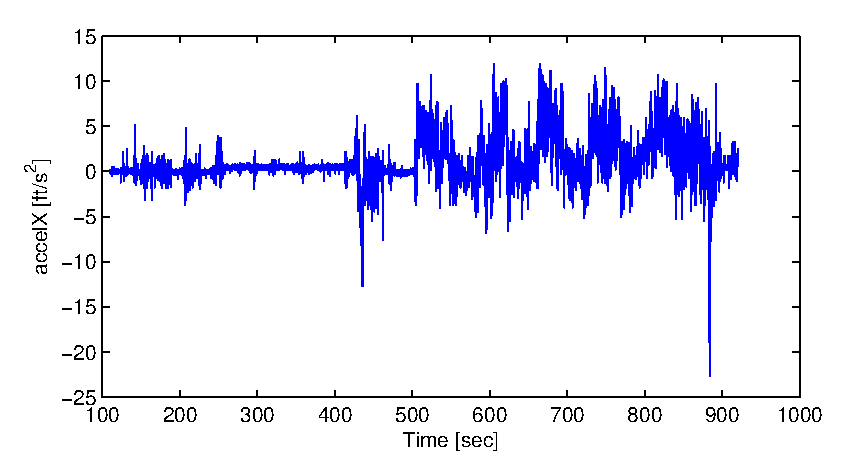
\includegraphics[width = 0.7\textwidth]{C:/Users/mufasa/Documents/Thesis/LaTex/figures/sampleOutput/accelX.eps}
\end{figure}
\begin{figure}[]
	\centering
	\caption{accelY vs. Time}
		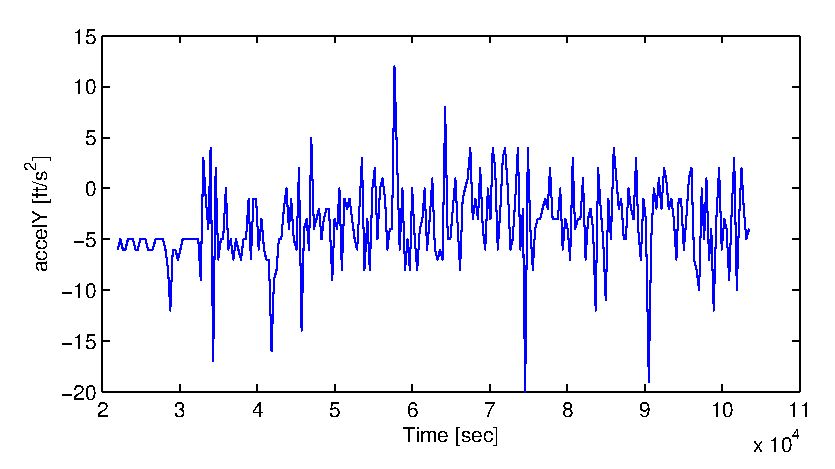
\includegraphics[width = 0.7\textwidth]{C:/Users/mufasa/Documents/Thesis/LaTex/figures/sampleOutput/accelY.eps}
\end{figure}
\begin{figure}[]
	\centering
	\caption{accelZ vs. Time}
		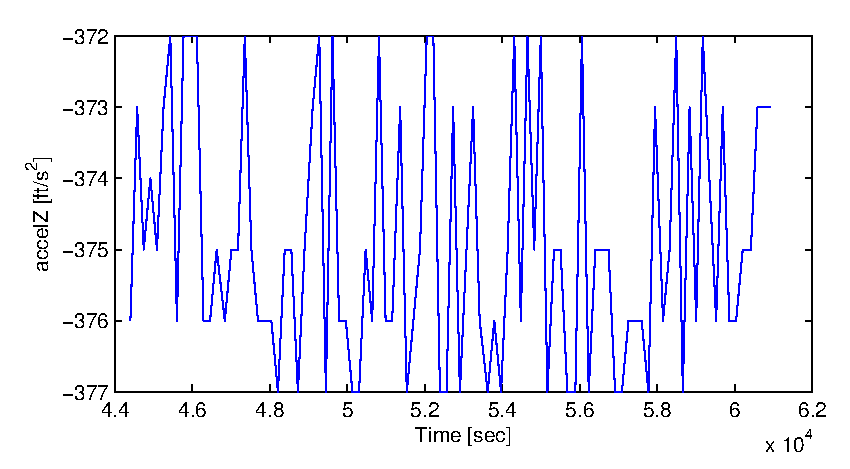
\includegraphics[width = 0.7\textwidth]{C:/Users/mufasa/Documents/Thesis/LaTex/figures/sampleOutput/accelZ.eps}
\end{figure}
\begin{figure}[]
	\centering
	\caption{gyroX vs. Time}
		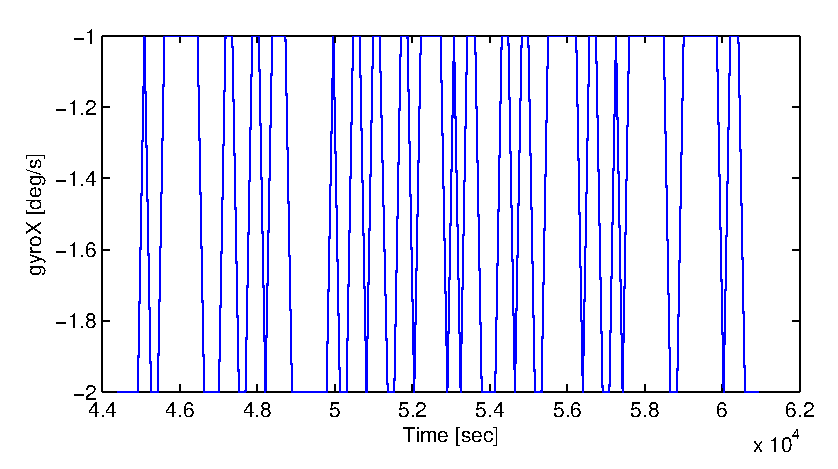
\includegraphics[width = 0.7\textwidth]{C:/Users/mufasa/Documents/Thesis/LaTex/figures/sampleOutput/gyroX.eps}
\end{figure}
\begin{figure}[]
	\centering
	\caption{gyroY vs. Time}
		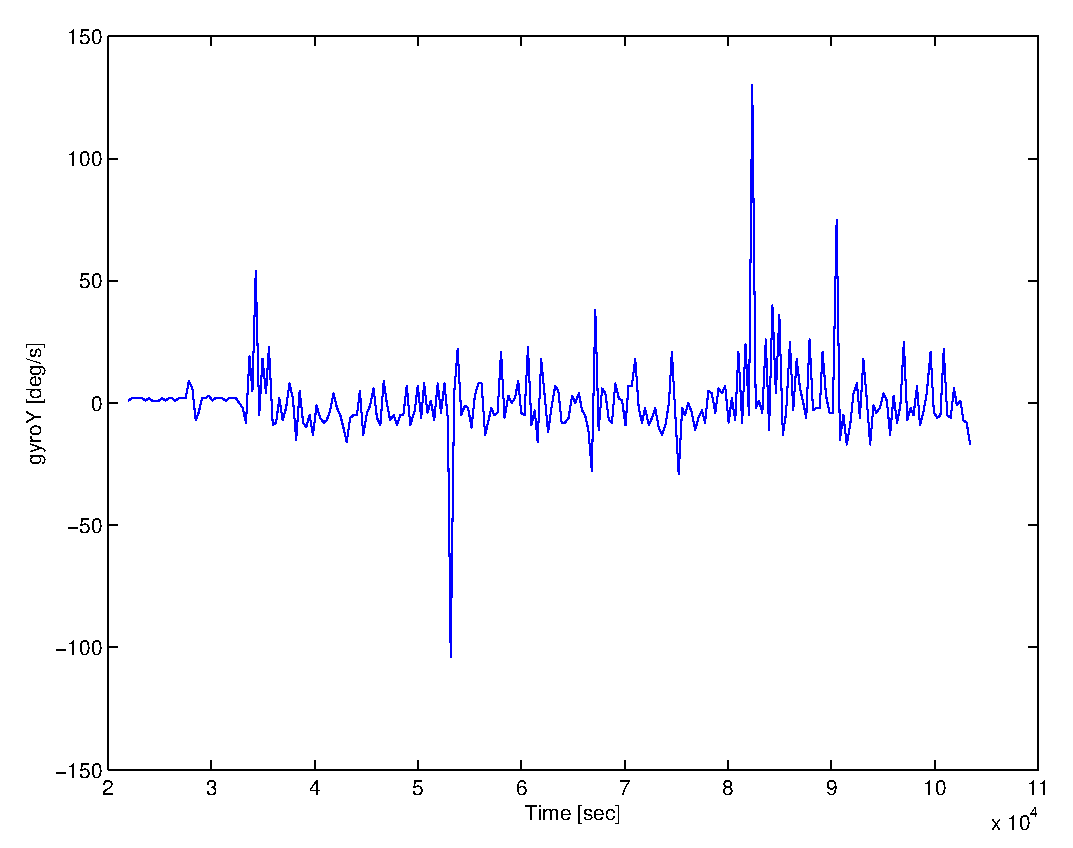
\includegraphics[width = 0.7\textwidth]{C:/Users/mufasa/Documents/Thesis/LaTex/figures/sampleOutput/gyroY.eps}
\end{figure}
\begin{figure}[]
	\centering
	\caption{gyroZ vs. Time}
		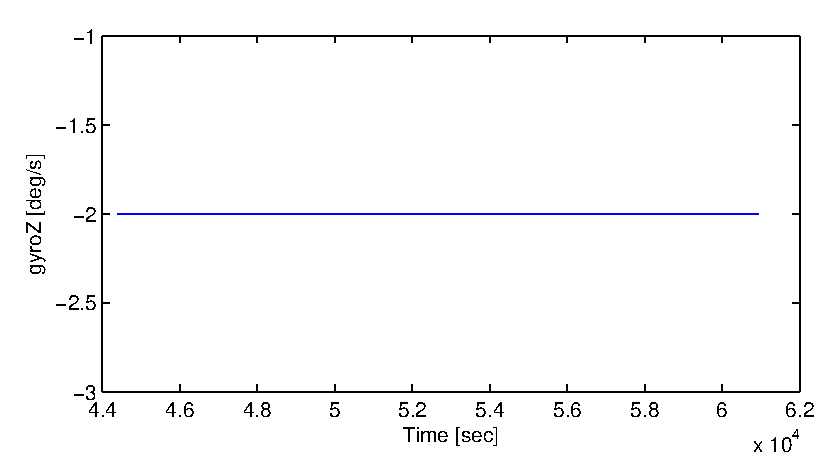
\includegraphics[width = 0.7\textwidth]{C:/Users/mufasa/Documents/Thesis/LaTex/figures/sampleOutput/gyroZ.eps}
\end{figure}
\begin{figure}[]
	\centering
	\caption{magX vs. Time}
		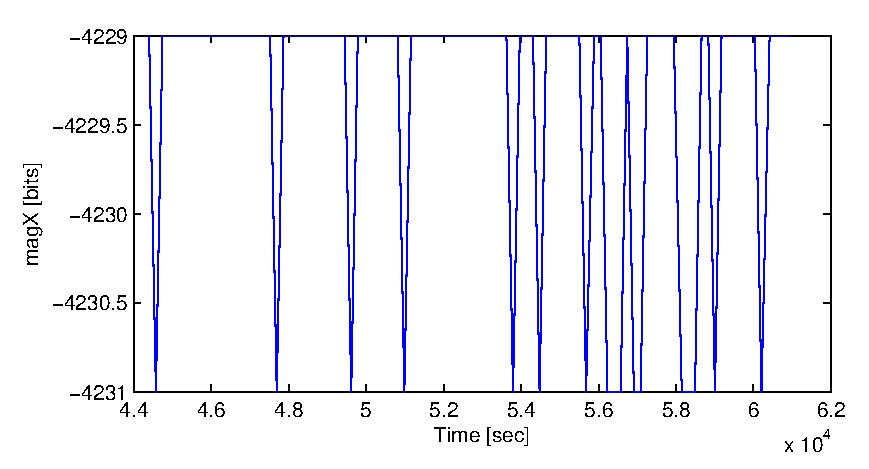
\includegraphics[width = 0.7\textwidth]{C:/Users/mufasa/Documents/Thesis/LaTex/figures/sampleOutput/magX.eps}
\end{figure}
\begin{figure}[]
	\centering
	\caption{magY vs. Time}
		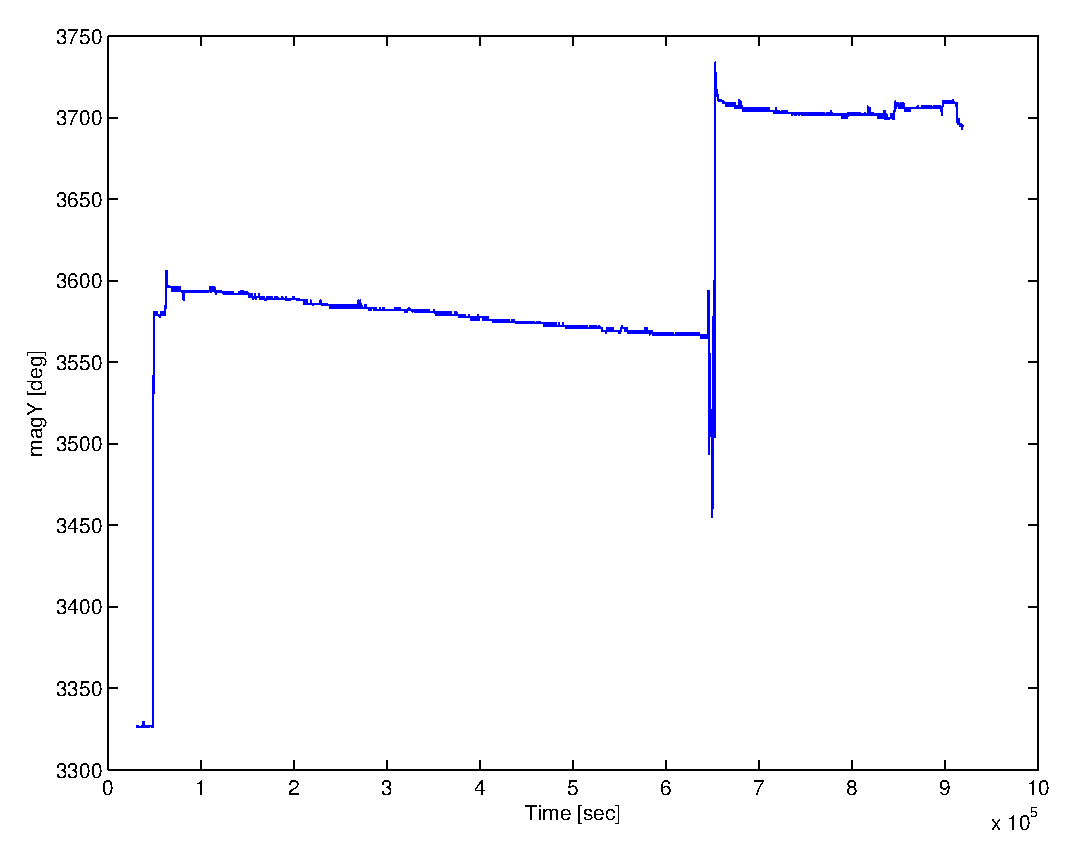
\includegraphics[width = 0.7\textwidth]{C:/Users/mufasa/Documents/Thesis/LaTex/figures/sampleOutput/magY.eps}
\end{figure}
\begin{figure}[]
	\centering
	\caption{magZ vs. Time}
		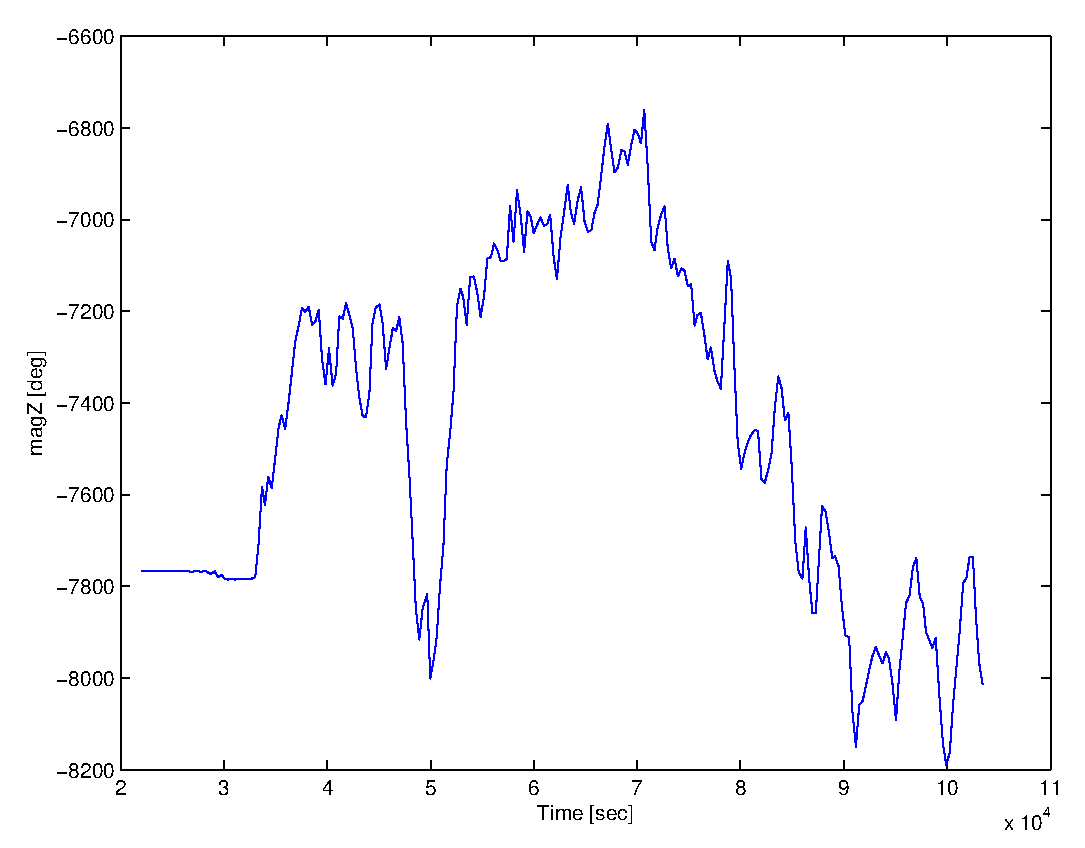
\includegraphics[width = 0.7\textwidth]{C:/Users/mufasa/Documents/Thesis/LaTex/figures/sampleOutput/magZ.eps}
\end{figure}
\begin{figure}[]
	\centering
	\caption{press0 vs. Time}
		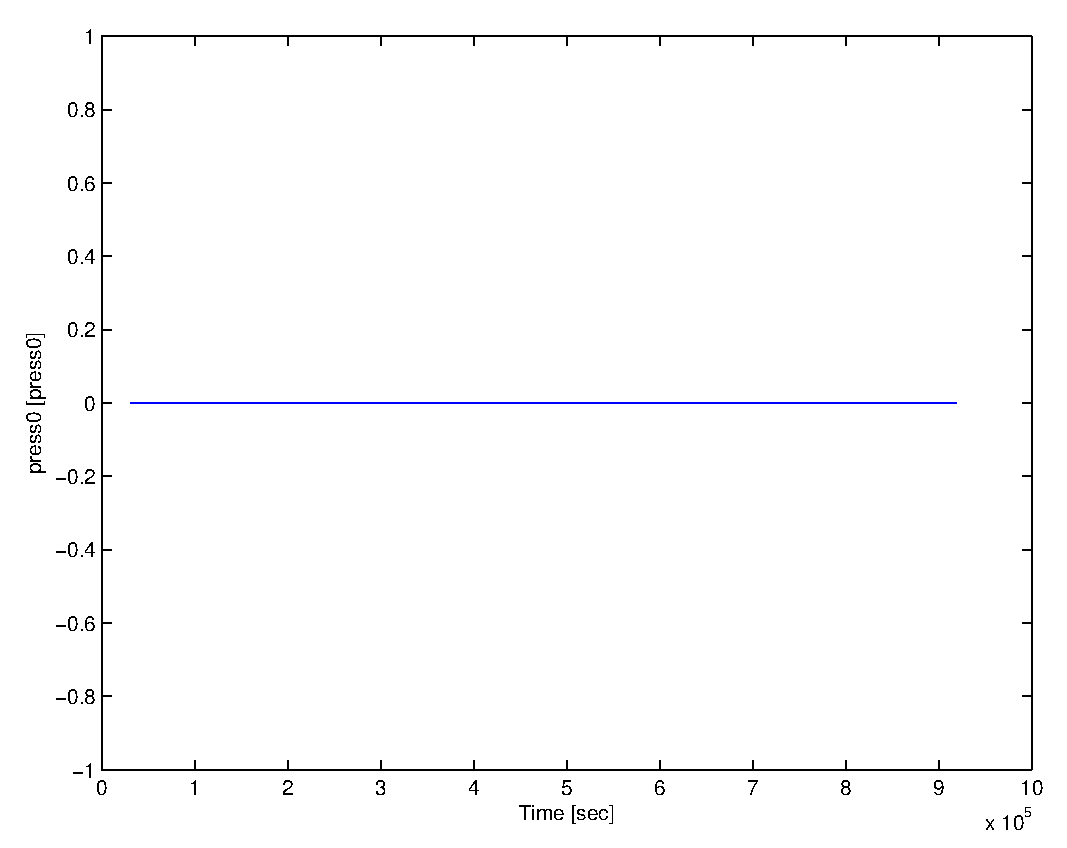
\includegraphics[width = 0.7\textwidth]{C:/Users/mufasa/Documents/Thesis/LaTex/figures/sampleOutput/press0.eps}
\end{figure}
\begin{figure}[]
	\centering
	\caption{press1 vs. Time}
		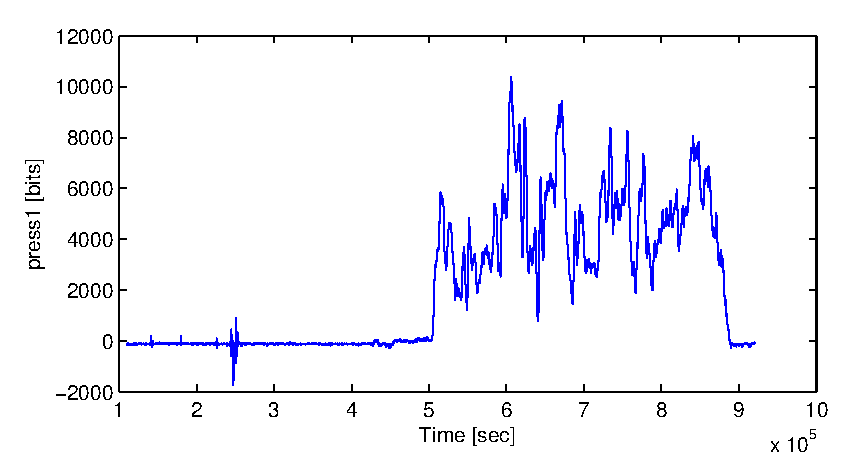
\includegraphics[width = 0.7\textwidth]{C:/Users/mufasa/Documents/Thesis/LaTex/figures/sampleOutput/press1.eps}
\end{figure}
\begin{figure}[]
	\centering
	\caption{press2 vs. Time}
		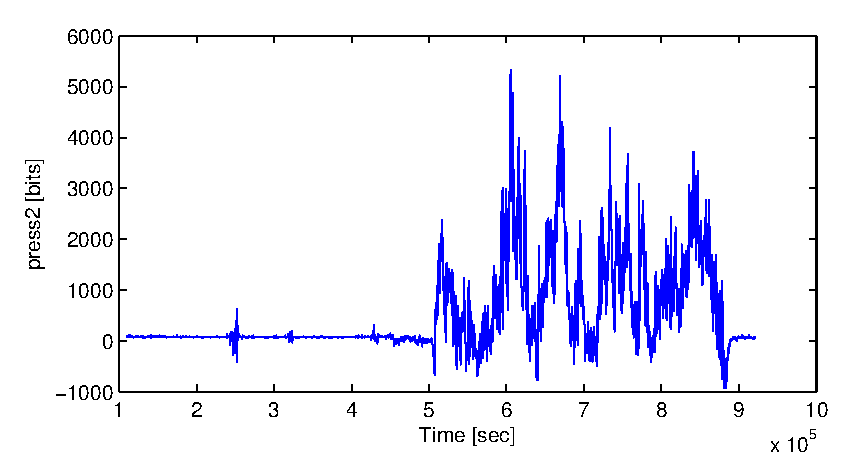
\includegraphics[width = 0.7\textwidth]{C:/Users/mufasa/Documents/Thesis/LaTex/figures/sampleOutput/press2.eps}
\end{figure}
\begin{figure}[]
	\centering
	\caption{press3 vs. Time}
		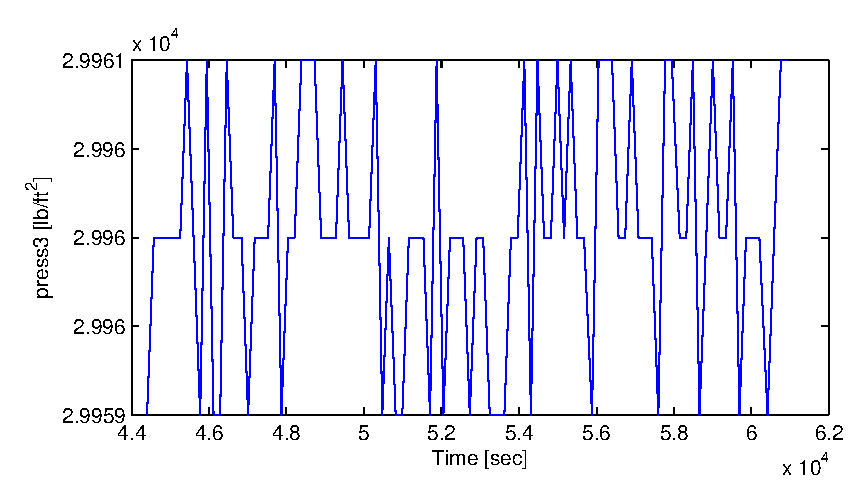
\includegraphics[width = 0.7\textwidth]{C:/Users/mufasa/Documents/Thesis/LaTex/figures/sampleOutput/press3.eps}
\end{figure}
\begin{figure}[]
	\centering
	\caption{gpsLat vs. Time}
		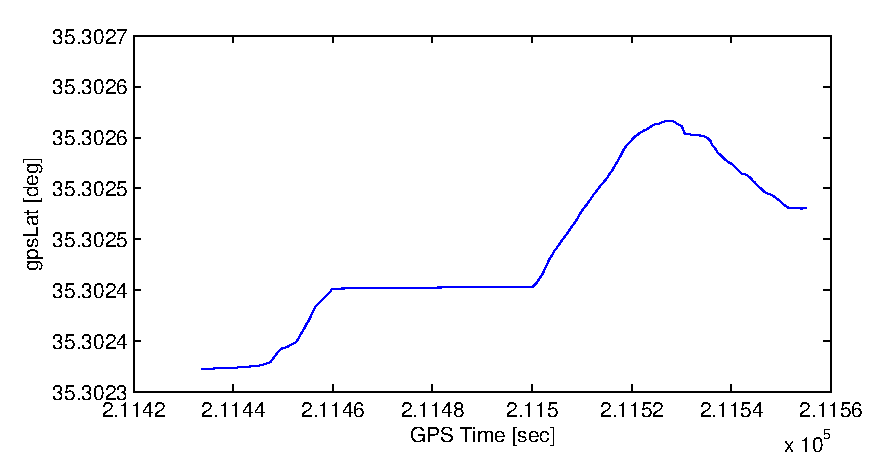
\includegraphics[width = 0.7\textwidth]{C:/Users/mufasa/Documents/Thesis/LaTex/figures/sampleOutput/gpsLat.eps}
\end{figure}
\begin{figure}[]
	\centering
	\caption{gpsLong vs. Time}
		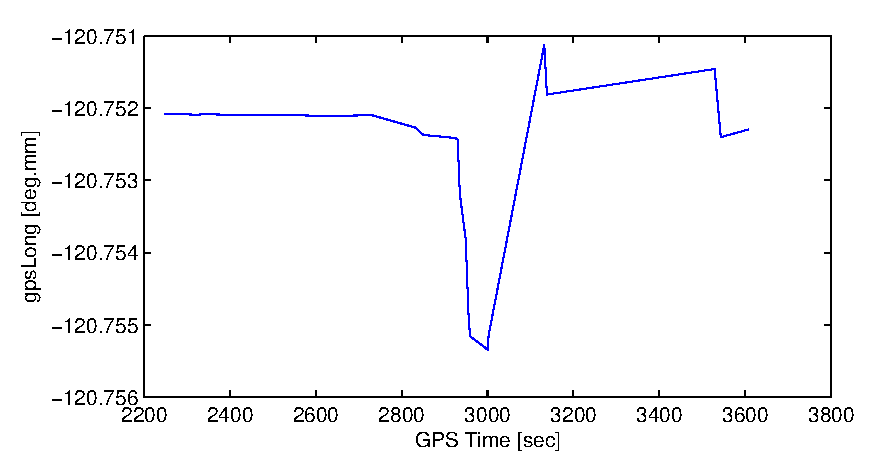
\includegraphics[width = 0.7\textwidth]{C:/Users/mufasa/Documents/Thesis/LaTex/figures/sampleOutput/gpsLong.eps}
\end{figure}
\begin{figure}[]
	\centering
	\caption{gpsSpd vs. Time}
		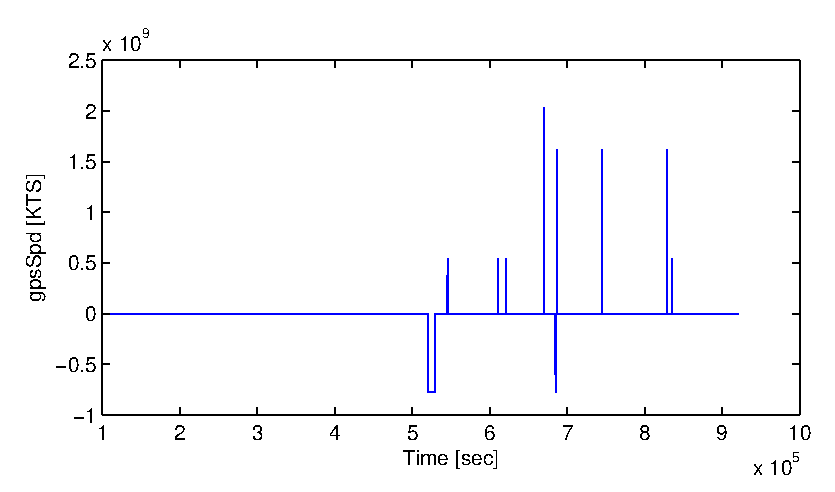
\includegraphics[width = 0.7\textwidth]{C:/Users/mufasa/Documents/Thesis/LaTex/figures/sampleOutput/gpsSpd.eps}
\end{figure}
\begin{figure}[]
	\centering
	\caption{gpsCrs vs. Time}
		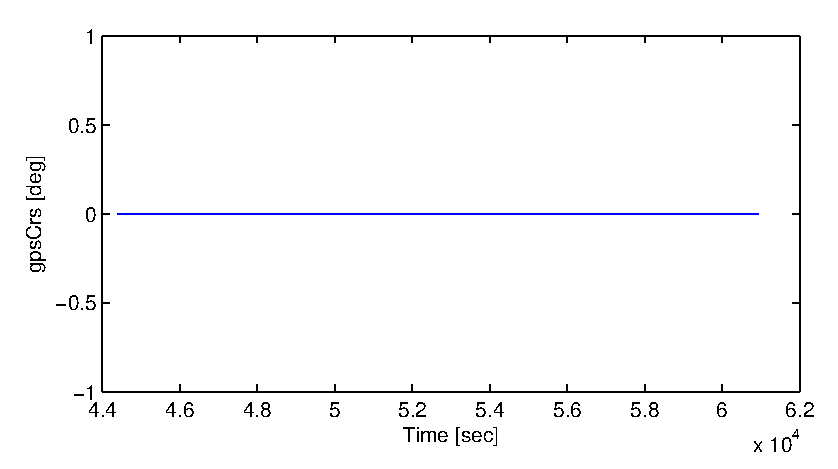
\includegraphics[width = 0.7\textwidth]{C:/Users/mufasa/Documents/Thesis/LaTex/figures/sampleOutput/gpsCrs.eps}
\end{figure}
\begin{figure}[]
	\centering
	\caption{date vs. Time}
		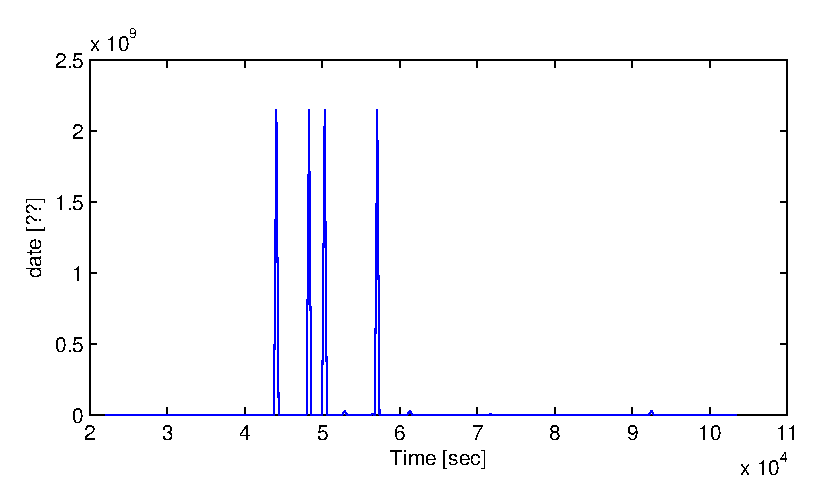
\includegraphics[width = 0.7\textwidth]{C:/Users/mufasa/Documents/Thesis/LaTex/figures/sampleOutput/date.eps}
\end{figure}
\begin{figure}[]
	\centering
	\caption{CS vs. Time}
		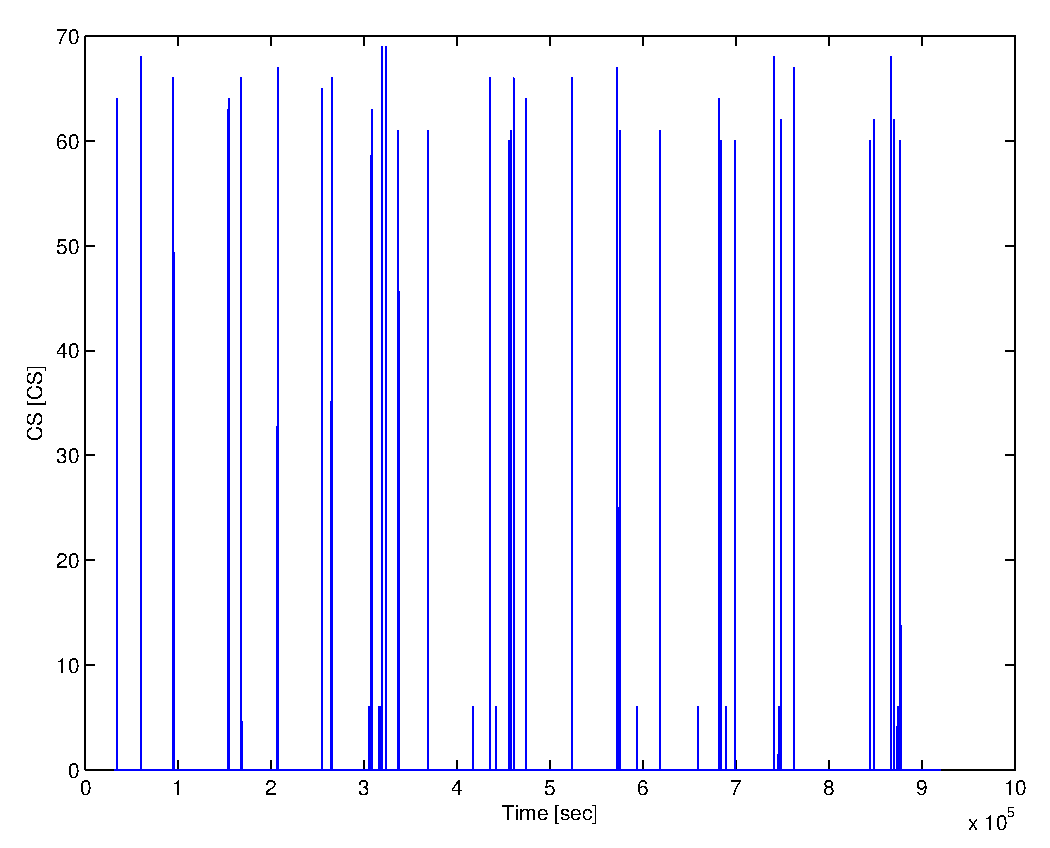
\includegraphics[width = 0.7\textwidth]{C:/Users/mufasa/Documents/Thesis/LaTex/figures/sampleOutput/CS.eps}
\end{figure}
\begin{figure}[]
	\centering
	\caption{temperature vs. Time}
		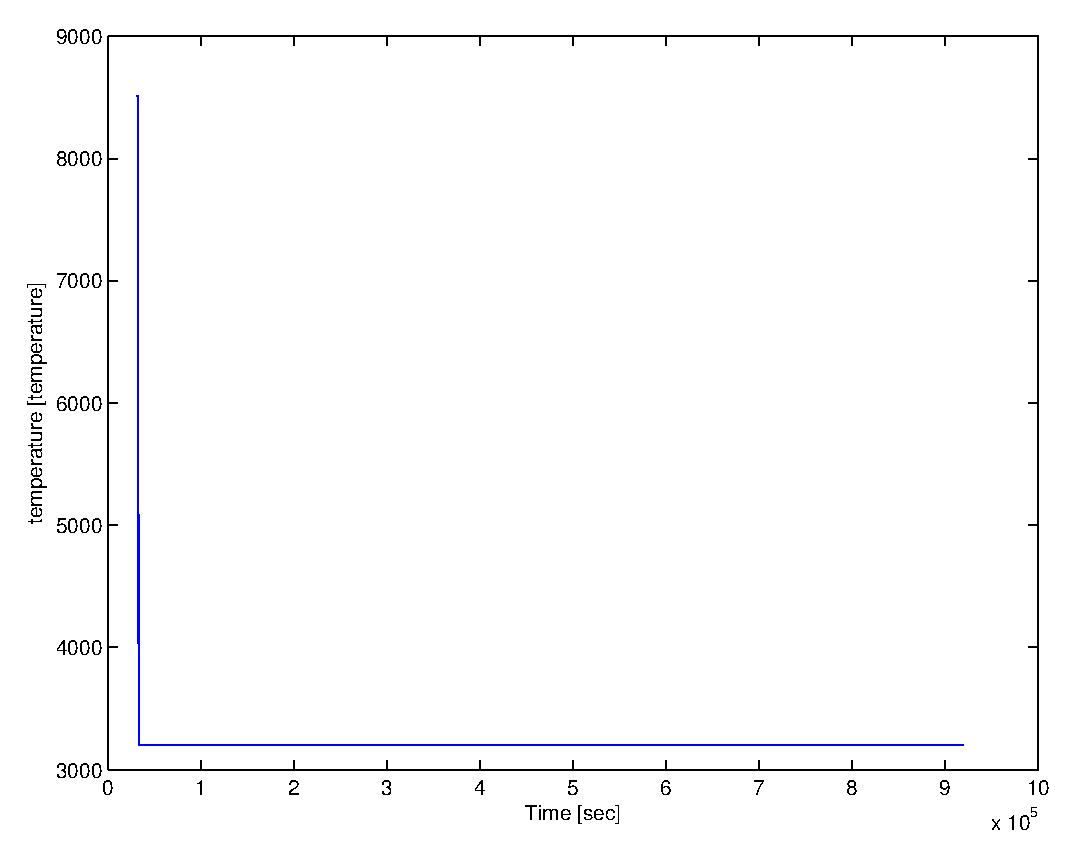
\includegraphics[width = 0.7\textwidth]{C:/Users/mufasa/Documents/Thesis/LaTex/figures/sampleOutput/temperature.eps}
\end{figure}
\begin{figure}[]
	\centering
	\caption{deltaT vs. Time}
		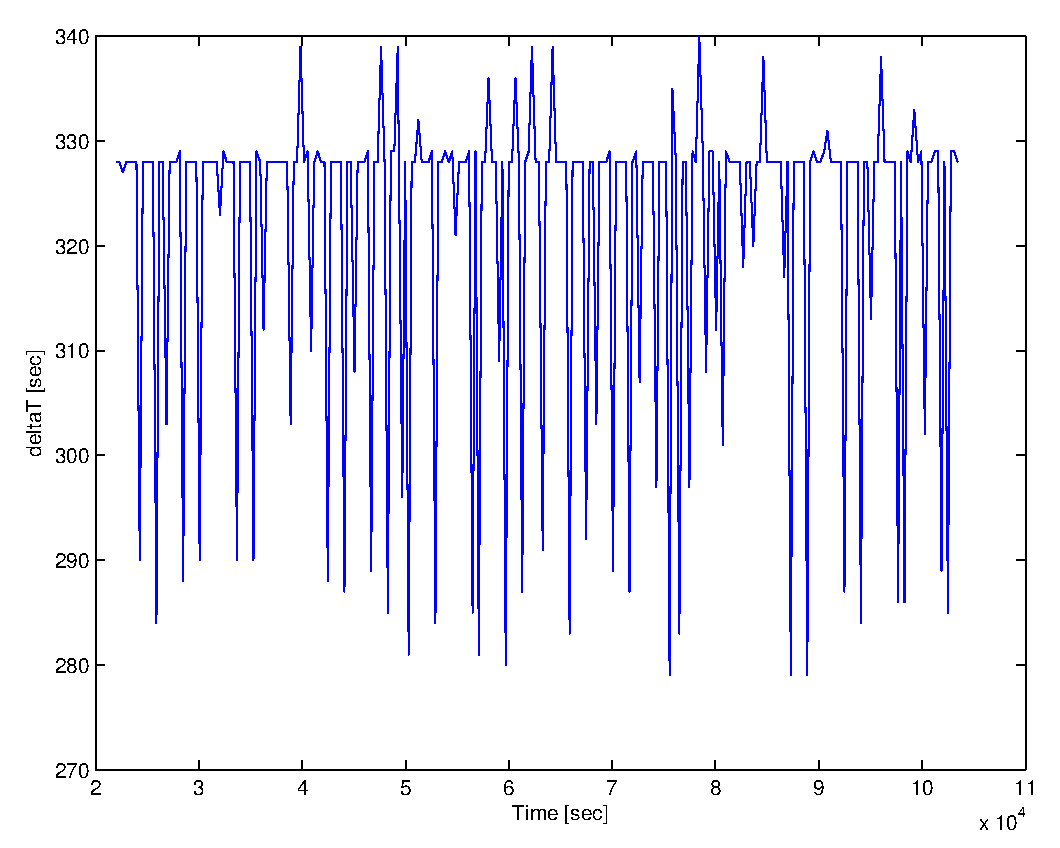
\includegraphics[width = 0.7\textwidth]{C:/Users/mufasa/Documents/Thesis/LaTex/figures/sampleOutput/deltaT.eps}
\end{figure}
\begin{figure}[]
	\centering
	\caption{alpha vs. Time}
		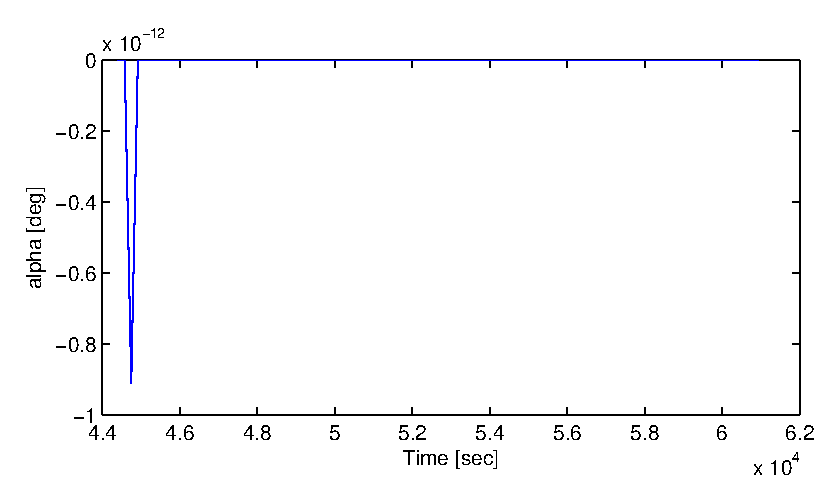
\includegraphics[width = 0.7\textwidth]{C:/Users/mufasa/Documents/Thesis/LaTex/figures/sampleOutput/alpha.eps}
\end{figure}
\begin{figure}[]
	\centering
	\caption{beta vs. Time}
		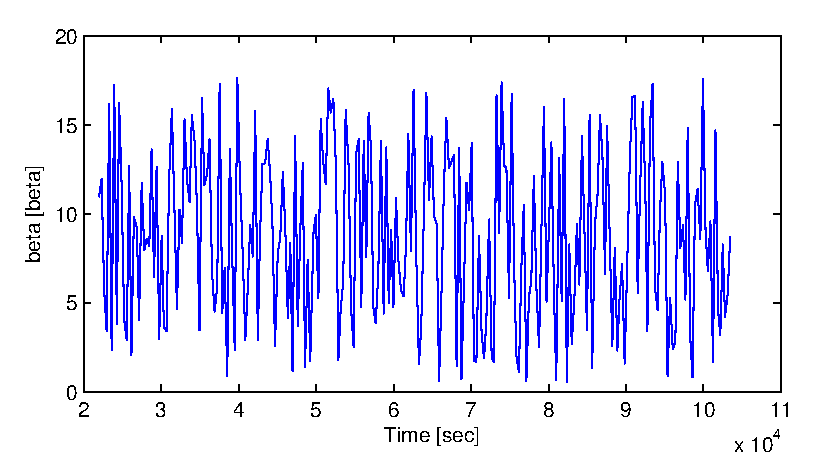
\includegraphics[width = 0.7\textwidth]{C:/Users/mufasa/Documents/Thesis/LaTex/figures/sampleOutput/beta.eps}
\end{figure}
\begin{figure}[]
	\centering
	\caption{ang1 vs. Time}
		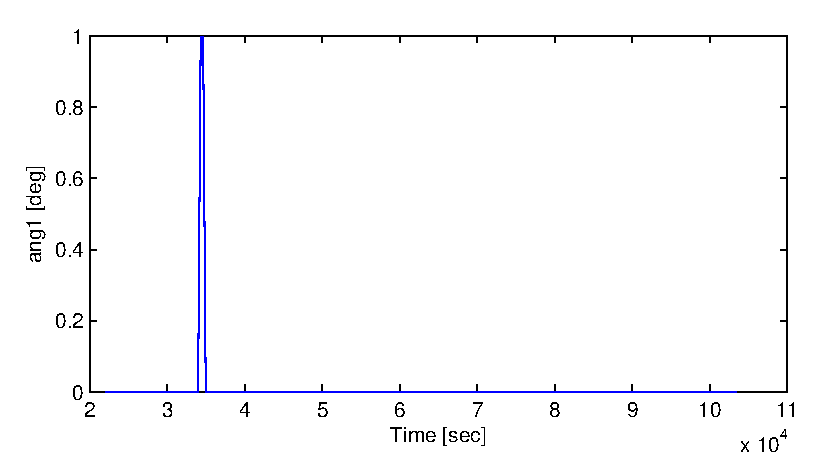
\includegraphics[width = 0.7\textwidth]{C:/Users/mufasa/Documents/Thesis/LaTex/figures/sampleOutput/ang1.eps}
\end{figure}
\begin{figure}[]
	\centering
	\caption{ang2 vs. Time}
		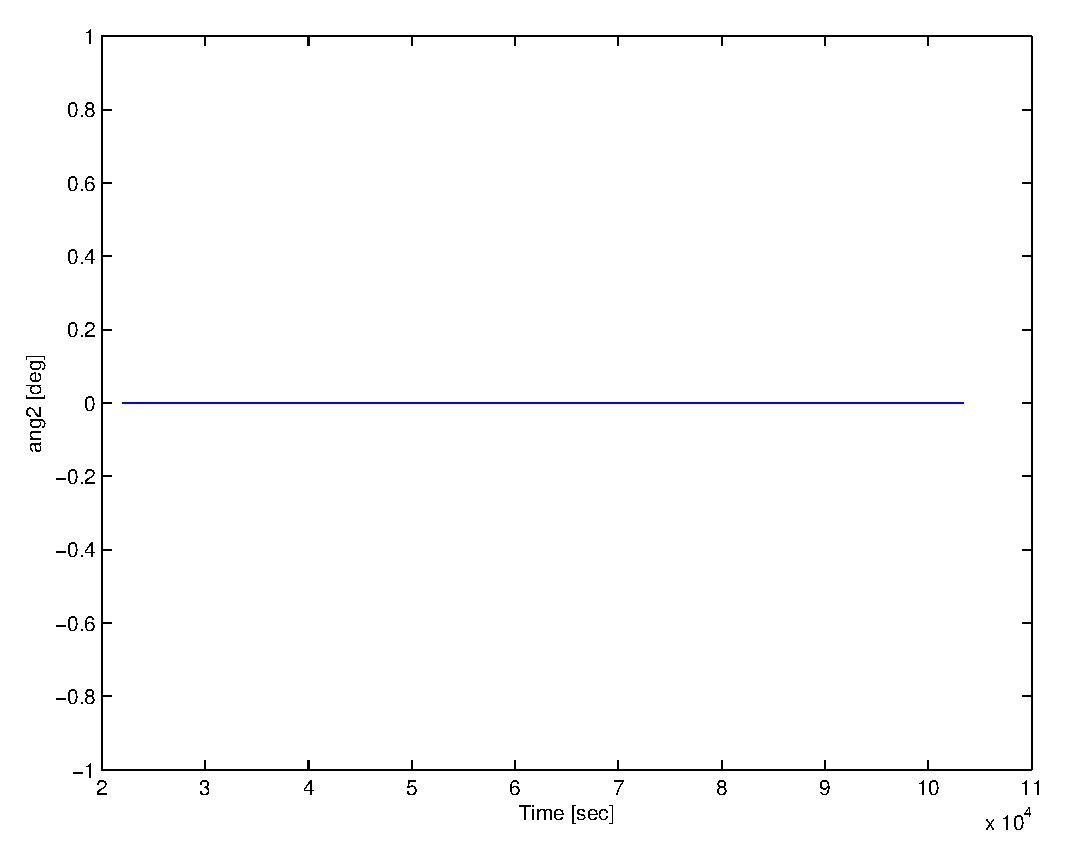
\includegraphics[width = 0.7\textwidth]{C:/Users/mufasa/Documents/Thesis/LaTex/figures/sampleOutput/ang2.eps}
\end{figure}
\begin{figure}[]
	\centering
	\caption{ang3 vs. Time}
		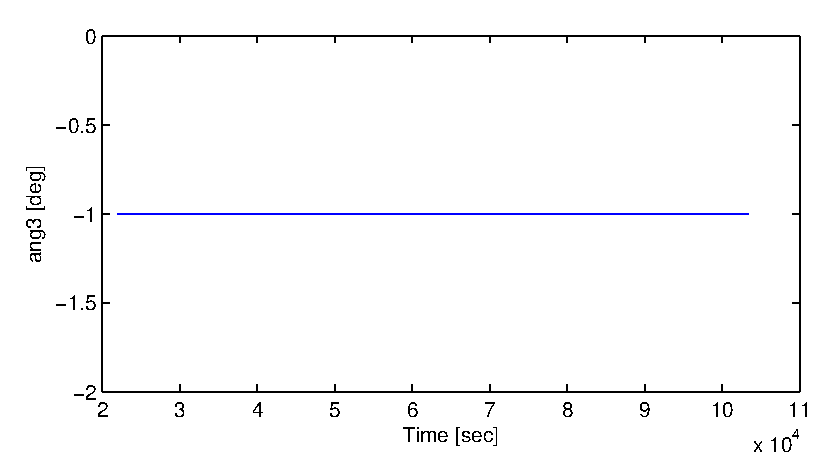
\includegraphics[width = 0.7\textwidth]{C:/Users/mufasa/Documents/Thesis/LaTex/figures/sampleOutput/ang3.eps}
\end{figure}
